%package list
\documentclass{article}
\usepackage{amsmath}
\usepackage[top=3cm, bottom=3cm, outer=3cm, inner=3cm]{geometry}
\usepackage{multicol}
\usepackage{graphicx}
\usepackage{url}
%\usepackage{cite}
\usepackage{hyperref}
\usepackage{array}
%\usepackage{multicol}
\newcolumntype{x}[1]{>{\centering\arraybackslash\hspace{0pt}}p{#1}}
\usepackage{natbib}
\usepackage{pdfpages}
\usepackage{multirow}
\usepackage[normalem]{ulem}
\useunder{\uline}{\ul}{}
\usepackage{svg}
\usepackage{xcolor}
\usepackage{minted}

%\usepackage{booktabs}
\usepackage{caption}
\usepackage{subcaption}
\usepackage{float}
\usepackage{array}

\newcolumntype{M}[1]{>{\centering\arraybackslash}m{#1}}
\newcolumntype{N}{@{}m{0pt}@{}}

%%%%%%%%%%%%%%%%%%%%%%%%%%%%%%%%%%%%%%%%%%%%%%%%%%%%%%%%%%%%%%%%%%%%%%%%%%%%
%%%%%%%%%%%%%%%%%%%%%%%%%%%%%%%%%%%%%%%%%%%%%%%%%%%%%%%%%%%%%%%%%%%%%%%%%%%%
\newcommand{\itemEmail}{ccapatinta@unsa.edu.pe}
\newcommand{\itemStudent}{Capatinta Almanza Camilo B. A.}
\newcommand{\itemCourse}{Lab. Análisis y Diseño de Algoritmos}
\newcommand{\itemCourseCode}{1702231}
\newcommand{\itemSemester}{IV}
\newcommand{\itemUniversity}{Universidad Nacional de San Agustín de Arequipa}
\newcommand{\itemFaculty}{Facultad de Ingeniería de Producción y Servicios}
\newcommand{\itemDepartment}{Departamento Académico de Ingeniería de Sistemas e Informática}
\newcommand{\itemSchool}{Escuela Profesional de Ingeniería de Sistemas}
\newcommand{\itemAcademic}{2026 - B}
\newcommand{\itemInput}{12/11/2026}
\newcommand{\itemOutput}{--/11/2026}
\newcommand{\itemPracticeNumber}{09}
\newcommand{\itemTheme}{Métodos Heurísticos: Heurísticas Constructivas y de Búsqueda Local.}
%%%%%%%%%%%%%%%%%%%%%%%%%%%%%%%%%%%%%%%%%%%%%%%%%%%%%%%%%%%%%%%%%%%%%%%%%%%%
%%%%%%%%%%%%%%%%%%%%%%%%%%%%%%%%%%%%%%%%%%%%%%%%%%%%%%%%%%%%%%%%%%%%%%%%%%%%

\usepackage[english,spanish]{babel}
\usepackage[utf8]{inputenc}
\AtBeginDocument{\selectlanguage{spanish}}
\renewcommand{\figurename}{Figura}
\renewcommand{\refname}{Referencias}
\renewcommand{\tablename}{Tabla} %esto no funciona cuando se usa babel
\AtBeginDocument{%
	\renewcommand\tablename{Tabla}
}

\usepackage{fancyhdr}
\pagestyle{fancy}
\fancyhf{}
\setlength{\headheight}{40.51407pt}
\renewcommand{\headrulewidth}{1pt}
\renewcommand{\footrulewidth}{1pt}
\fancyhead[L]{\raisebox{-0.2\height}{\includegraphics[width=3cm]{../img/logo_episunsa.png}}}
\fancyhead[C]{\fontsize{7}{7}\selectfont	\itemUniversity \\ \itemFaculty \\ \itemDepartment \\ \itemSchool \\ \textbf{\itemCourse}}
\fancyhead[R]{\raisebox{-0.2\height}{\includegraphics[width=1.2cm]{../img/logo_abet}}}
\fancyfoot[L]{Estudiante Capatinta C.}
\fancyfoot[C]{\itemCourse}
\fancyfoot[R]{Página \thepage}

% para el codigo fuente

\usepackage{color, colortbl}
\definecolor{dkgreen}{rgb}{0,0.6,0}
\definecolor{gray}{rgb}{0.5,0.5,0.5}
\definecolor{mauve}{rgb}{0.58,0,0.82}
\definecolor{codebackground}{rgb}{0.95, 0.95, 0.92}
\setminted{%
  fontsize=\small,
  breaklines,
  linenos,
  numbersep=6pt,
  frame=lines,
  framesep=3mm,
  baselinestretch=1,
  bgcolor=codebackground,
  tabsize=3
}
\definecolor{tablebackground}{rgb}{0.8, 0, 0}

\begin{document}
	
	\vspace*{10px}
	
	\begin{center}
		\parbox{0.8\textwidth}{\centering\fontsize{17}{20}\selectfont\textbf{Informe de laboratorio \itemPracticeNumber}}
	\end{center}
	\begin{center}
		\parbox{0.8\textwidth}{\centering\textbf{\Large Tema: \itemTheme}}
	\end{center}
	%\vspace*{0.5cm}	

	\begin{flushright}
		\begin{tabular}{|M{2.5cm}|N|}
			\hline 
			\rowcolor{tablebackground}
			\color{white} \textbf{Nota}  \\
			\hline 
			     \\[30pt]
			\hline 			
		\end{tabular}
	\end{flushright}	

	\begin{table}[h!]
		\begin{tabular}{|x{4.7cm}|x{4.8cm}|x{4.8cm}|}        
			\hline 
			\rowcolor{tablebackground}
			\color{white} \textbf{Estudiante} & \color{white}\textbf{Escuela}  & \color{white}\textbf{Asignatura}   \\
			\hline 
			{\itemStudent \par \itemEmail} & \itemSchool & {\itemCourse \par Semestre: \itemSemester \par Código: \itemCourseCode}     \\
			\hline 			
		\end{tabular}
	\end{table}		
	
	\begin{table}[H]
		\begin{tabular}{|x{4.7cm}|x{4.8cm}|x{4.8cm}|}
			\hline 
			\rowcolor{tablebackground}
			\color{white}\textbf{Laboratorio} & \color{white}\textbf{Tema}  & \color{white}\textbf{Duración}   \\
			\hline 
			\itemPracticeNumber & \itemTheme & 02 horas   \\
			\hline 
		\end{tabular}
	\end{table}
	
	\begin{table}[H]
		\begin{tabular}{|x{4.7cm}|x{4.8cm}|x{4.8cm}|}
			\hline 
			\rowcolor{tablebackground}
			\color{white}\textbf{Semestre académico} & \color{white}\textbf{Fecha de inicio}  & \color{white}\textbf{Fecha de entrega}   \\
			\hline 
			\itemAcademic & \itemInput &  \itemOutput  \\
			\hline 
		\end{tabular}
	\end{table}
	
\section{Ejercicios propuestos por el docente}

\subsection{Construcción de una ruta con Nearest Neighbor}
Construir una ruta para el TSP de cinco ciudades del Laboratorio 8 usando la misma matriz de distancias. Aplicar Nearest Neighbor empezando en la ciudad 0 y comparar el costo obtenido con el óptimo conocido, que es 70.

\inputminted{cpp}{../e-p/tsp_nearest_neighbor.cpp}

\begin{figure}[H]
    \centering
    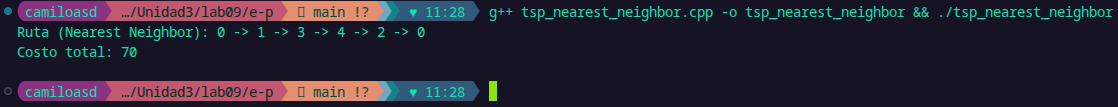
\includegraphics[width=0.9\textwidth]{../img/nn.png}
    \caption{Ruta para el TSP de 5 ciudades.}
    \label{fig:nn}
\end{figure}

La heurística comienza en la ciudad 0 y, en cada paso, elige la ciudad no visitada más cercana a la ciudad actual. Cuando todas las ciudades han sido visitadas, cierra el recorrido regresando al origen. El programa almacena las distancias en una matriz y usa un vector para marcar las ciudades visitadas y otro para construir la ruta. Para esta instancia obtiene la ruta 0--1--3--4--2--0, de costo 70.

\subsection{Mejora de una ruta con búsqueda local 2-opt}

Aplicar 2-opt a la ruta inicial 0--1--2--4--3--0, obtenida con Nearest Neighbor al empezar en la ciudad 2, cuyo costo es 85. Comparar la ruta mejorada con el óptimo conocido del TSP, de costo 70.

\inputminted{cpp}{../e-p/tsp_2opt.cpp}

\begin{figure}[H]
    \centering
    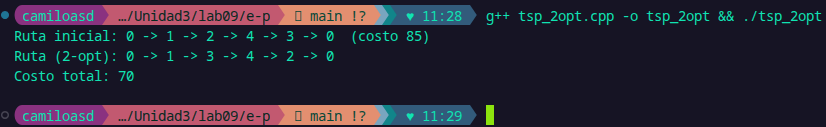
\includegraphics[width=0.9\textwidth]{../img/2opt.png}
    \caption{Ruta mejorada con 2-opt.}
    \label{fig:2-opt}
\end{figure}

El algoritmo parte de una ruta completa y prueba invertir segmentos entre distintas posiciones. Calcula el costo de cada ruta candidata y acepta una inversión solo cuando reduce estrictamente el costo. Repite las pruebas hasta que ninguna inversión produzca una mejora. En este ejemplo invierte un segmento y obtiene la ruta 0--1--3--4--2--0, reduciendo el costo de 85 a 70.

\section{Ejercicios/Problemas propuestos}

\subsection{Header compartido: tsp.h}
Reúne tipos, datos y funciones comunes para todos los ejercicios, se incorporan en estos mediante \texttt{\#include "tsp.h"}. Calcula costos y aplica las heurísticas Nearest Neighbor y 2-opt. Contiene también funciones para generar instancias aleatorias de TSP y para medir tiempos de ejecución.
\inputminted{cpp}{../e-n/tsp.h}

\subsection{Ejercicio 1}
Implementa Nearest Neighbor para un TSP de 15 ciudades generadas aleatoriamente, y ejecútalo partiendo de cada una de las 15 ciudades como origen. ¿El resultado cambia según el punto de partida?
\inputminted{cpp}{../e-n/e1.cpp}

\begin{itemize}
    \item /relleno
\end{itemize}

\begin{figure}[H]
    \centering
    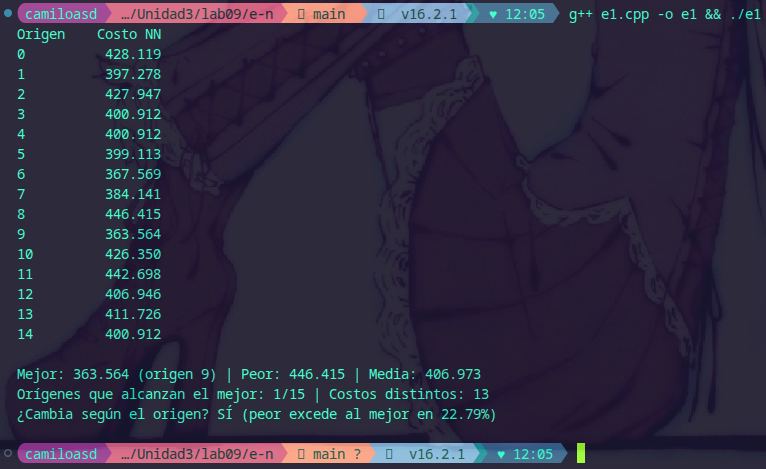
\includegraphics[width=0.8\textwidth]{../img/e1.png}
    \caption{Ejecución del ejercicio 1}
    \label{fig:e1}
\end{figure}

\subsection{Ejercicio 2}
Aplica 2-opt sobre las 15 soluciones del ejercicio anterior. ¿El mejor resultado final sigue dependiendo de la ciudad de origen usada por Nearest Neighbor?
\inputminted{cpp}{../e-n/e2.cpp}

\begin{itemize}
    \item /relleno
\end{itemize}

\begin{figure}[H]
    \centering
    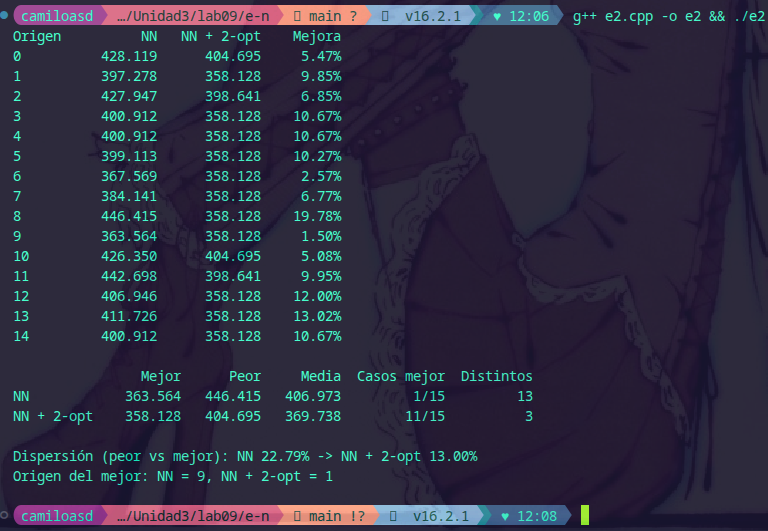
\includegraphics[width=0.8\textwidth]{../img/e2.png}
    \caption{Ejecución del ejercicio 2}
    \label{fig:e2}
\end{figure}

\subsection{Ejercicio 3}
Implementa otra heurística constructiva: la heurística del "vecino más barato" (cheapest insertion), que en cada paso inserta la ciudad no visitada que menos aumenta el costo total, en cualquier posición de la ruta. Compárala contra Nearest Neighbor.
\inputminted{cpp}{../e-n/e3.cpp}

\begin{itemize}
    \item /relleno
\end{itemize}

\begin{figure}[H]
    \centering
    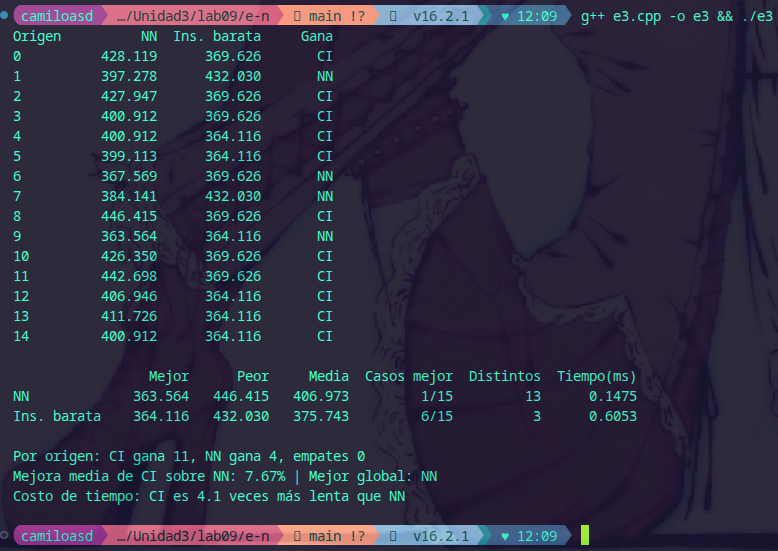
\includegraphics[width=0.8\textwidth]{../img/e3.png}
    \caption{Ejecución del ejercicio 3}
    \label{fig:e3}
\end{figure}

\subsection{Ejercicio 4}
Mide el tiempo de ejecución de Nearest Neighbor + 2-opt para instancias de 20, 50 y 100 ciudades, y compáralo contra el tiempo que tomaría fuerza bruta para esos mismos tamaños (estimado, sin ejecutarlo).
\inputminted{cpp}{../e-n/e4.cpp}

\begin{itemize}
    \item /relleno
\end{itemize}

\begin{figure}[H]
    \centering
    \includegraphics[width=0.8\textwidth]{../img/e4.png}
    \caption{Ejecución del ejercicio 4}
    \label{fig:e4}
\end{figure}

\subsection{Ejercicio 5}
Aplica Nearest Neighbor + 2-opt a un caso real: una lista de direcciones o puntos de interés de tu ciudad (puedes usar coordenadas aproximadas), y calcula la ruta de reparto o visita más corta posible.
\inputminted{cpp}{../e-n/e5.cpp}

\begin{itemize}
    \item /relleno
\end{itemize}

\begin{figure}[H]
    \centering
    \includegraphics[width=0.8\textwidth]{../img/e5.png}
    \caption{Ejecución del ejercicio 5}
    \label{fig:e5}
\end{figure}

\section{Cuestionario}
\begin{itemize}
	\item ¿Cuál es la diferencia entre un método aproximado y un método heurístico?
	\item ¿Por qué Nearest Neighbor puede terminar con un salto muy costoso al final de la ruta? Usa como ejemplo el inicio en la ciudad 2 de la Tabla 3.
	\item ¿Qué significa que 2-opt encuentre un "óptimo local"? ¿Por qué no garantiza el óptimo global?
	\item ¿Por qué combinar una heurística constructiva con una de búsqueda local suele dar mejores resultados que usar cualquiera de las dos por separado?
	\item Comparando la Figura 5 (y la Tabla 5) de este laboratorio con lo visto en el Laboratorio 8, ¿por qué Nearest Neighbor + 2-opt es preferible a Monte Carlo incluso con un presupuesto de cómputo similar?
\end{itemize}

\section{Conclusiones}
% Pendiente de completar.

	%\begin{itemize}	
	%	\item Se creo el archivo \textbf{.gitignore} para no considerar los archivos %\textbf{*.class} que son innecesarios hacer seguimiento.
	%\end{itemize}
	%\begin{lstlisting}[language=bash]
	%	$ vim lab01/.gitignore
	%\end{lstlisting}
	%\begin{lstlisting}[language=bash]
	%	*.class
	%\end{lstlisting}
	%\begin{lstlisting}[language=bash]
	%	$ git add .
	%	$ git commit -m "Creando .gitignore para archivos *.class"			
	%	$ git push -u origin main
	%\end{lstlisting}
	
	%\begin{lstlisting}[language=bash]
	%	$ vim lab01/Insertion.java
	%\end{lstlisting}
	
    
%\clearpage
%\bibliographystyle{apalike}
%\bibliographystyle{IEEEtranN}
%\bibliography{bibliography}
			
\end{document}\noindent\textbf{Enunciado:}
